\documentclass{article}
\usepackage[utf8]{inputenc}
\usepackage{algorithm}
\usepackage{algorithmic}
\usepackage{graphicx} % more modern
\usepackage{subfigure} 
\usepackage{times}
\usepackage{helvet}
\usepackage{courier}
\usepackage{numberedblock}
\setlength\blockindent{0.0in}
\usepackage{hyperref}

\hypersetup{
    colorlinks=true,
    linkcolor=blue,
    filecolor=magenta,      
    urlcolor=cyan,
}

\title{Use LSTMs to Write Your Own Sherlock Novel}
\author{Cat McQueen}

\begin{document}

\maketitle

\tableofcontents

\section{Get Started on Google Colab}

Google Colab is an environment that allows you to do Machine and Deep Learning for free. It can be connected to GitHub and has GPUs that you can use for free. It runs as a Jupyter notebook.

Google Colab is found at https://colab.research.google.com and requires a gmail account. Sign into your gmail account and it will open a pop-up. 
In the bottom right corner, select "NEW NOTEBOOK".

The window should appear the same as Figure~\ref{fig:home}

\begin{figure}[h!]
\centering
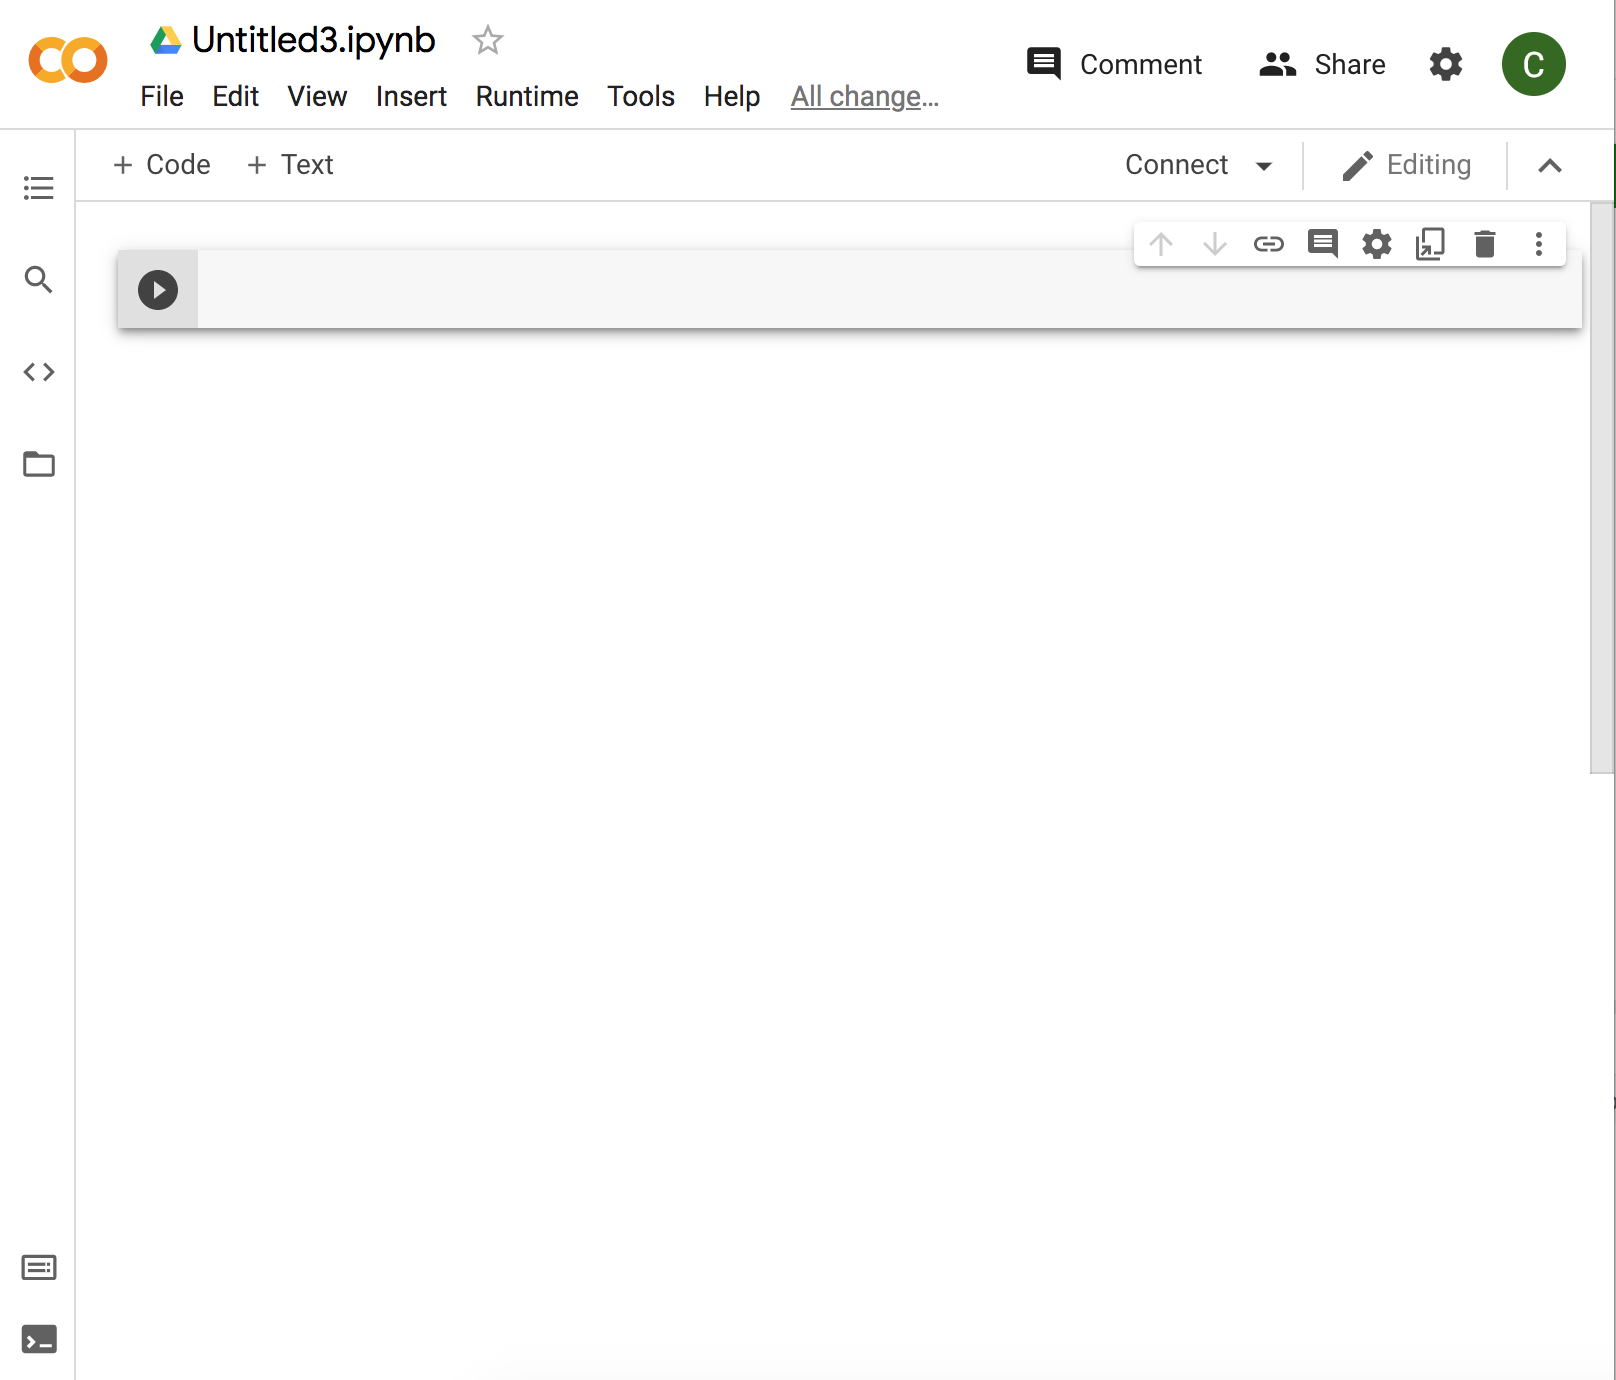
\includegraphics[width=50mm]{ColabHome.png}
\caption{Colab Homepage}
\label{fig:home}
\end{figure}

Now that we're on the right location, we can start coding!

\section{Import data}

The first thing we are going to do is import our Sherlock text file. Sherlock Holmes written by Conan Doyle is now in the public domain and is a dataset we can use to train. This is important to note: you cannot train networks for public consumption on texts that are currently copyrighted.

\subsection{Method 1 (Temporary Upload):} 

To download for this session only (the session will time out after some period of inactivity on the page).

First, download the data onto your local system by downloading 
\href{https://github.com/CatMcQueen/catmcqueen.github.io/blob/b67a282c9be6bfd1ed17796c2507b9108cffb6bc/sherlock.txt}{the Sherlock Text}. On the webpage, on the right, there is a Download button that will allow you to download this text.

Then, we are going to import it into our local Colab you have started. On the side of your colab noteboook, you will see a file icon (the fourth icon down on the left bar), if you click on it you will see a folder location. In order to connect to the folder location, you need to be connected to the runtime, which requires you run something. To get the file folder connected, type
\begin{verbatim}
print('hello world')
\end{verbatim} 
Then while still inside the text box, press shift and Enter. This will run the code within the box you are currently in.

Repeat every new Run time:
You will then see an empty folder path. We are going to upload sherlock.txt to our setup so we can call it in our python script.

\begin{figure}[h!]
\centering
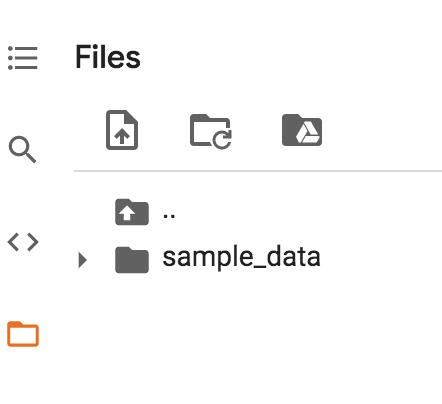
\includegraphics[width=50mm]{FileFolder.png}
\caption{The File Upload Bar}
\label{fig:filefolder}
\end{figure}

Click on the upload icon, and upload the sherlock.txt you previously downloaded to your local system. Now we're ready to read it in and parse the data.

\begin{figure}[h!]
\centering

\includegraphics[width=50mm]{GoogleDriveConnect.png}
\caption{Select Connect to Google Drive}
\label{fig:connectdrive}
\end{figure}

\subsection{Method 2 Google Drive:}

First, download the data onto your local system by downloading 
\href{https://github.com/CatMcQueen/catmcqueen.github.io/blob/b67a282c9be6bfd1ed17796c2507b9108cffb6bc/sherlock.txt}{the Sherlock Text}. On the webpage, on the right, there is a Download button that will allow you to download this text.

To upload so the file can be read indefinitely, we'll mount our google drive inline and upload the file from there. First, click on the right Google Drive icon on the file upload page shown in Figure~\ref{fig:filefolder}. You will then see a window pop up asking you to permit it to access your Drive. It may require you to register using an access code the first time. When you see Figure~\ref{fig:connectdrive} pop up, select Connect to Google Drive. Run

\begin{verbatim}
%cd drive/My Drive/
\end{verbatim}

If you have saved sherlock.txt within another folder in Google Drive, append the folder path to the path in the cd command. We will now be able to run our script even after the runtime disconnects without loading sherlock.txt again.

\subsection{Method 3 (Recommended):}

We are going to do a git checkout from this repository of just the sherlock.txt. This link can be found by going to \href{https://github.com/CatMcQueen/catmcqueen.github.io/blob/main/sherlock.txt}{the Sherlock Text} and copying the permalink from that webpage.

\begin{verbatim}
!git clone -n \ 
https://github.com/CatMcQueen/catmcqueen.github.io.git 
--depth 1
%cd catmcqueen.github.io
!git checkout HEAD sherlock.txt
\end{verbatim}

This will checkout the file sherlock.txt from the repository, and allow us to call it in our local system. Since it is part of our code, it will check it out every time we run through the code; therefore, it does not require we reload data every runtime. It also does not require you to ever download sherlock.txt to your own machine or Google Drive.  

\section{Read and Process File}

The first thing we are going to do is to read the text file in, and look at the data given. Now that we have the sherlock.txt in our local runtime, read the file into a variable. Remember to close the file after loading the data.

\begin{verbatim}
# Open a file: sherlock.txt in read mode
file = open('sherlock.txt',mode='r')
 
# read all lines into sherlock_txt
sherlock_txt = file.read()
 
# close the file
file.close()
\end{verbatim}

Now that you have the file, we are going to process it. This entails
1) removing punctuation and numbers, 2) removing any unnecessary white space, 3) reformatting into sentences, instead of lines. Once the data is processed, we can tokenize it and begin to use the data.

\subsection{1: Removing White Space and Punctuation}

Since we read the file in from text, there is a chance there is both leading white space(at the beginning of the file) and empty lines. We read the file in all at once, so we are going to process the text as a whole. 

\subsection{Remove all Leading White Space:}

To remove the leading white space at the beginning of the file (we don't want our first token to be a space), we will run a regular expression to eliminate it.
\begin{verbatim}
import re
sherlock_text1  = re.sub('^\s+', '', sherlock_txt)
\end{verbatim}

re allows us to do a substitution, with re(x, y) replacing anything matching the x pattern with y. The carat in regular expressions represents a new line, and the s is all spaces, with the + meaning that there has to be at least 1 for it to match. This regular expression, then, is replacing anything number of spaces at the beginning of the file with an empty vector. In practice, this removes all leading space characters. 

\subsection{Remove all Formatting Spaces:}

Next we'll remove all tabs, empty lines, and other forms of white space and replace them with a single space. Since tokenizing often breaks on spaces, a single space between words is the standard. In the same fashion as before, we'll use re.sub.
\begin{verbatim}
sherlock_text2 = re.sub(r'\s+', ' ', sherlock_text1)
\end{verbatim}
 In this case, r' means to not use the backslash as a literal character, but to use it as part of the spaces. 
 \begin{verbatim}
'\s+'
 \end{verbatim}
 represents all whitespaces, so we are replacing all white spaces with a single space.
 
 \subsection{Remove all Punctuation:}
 
 When we are generating text, we will not use this; however, for analyzing what words are most used and learning the data, we will want to remove punctuation, as they are the most common "words" in our corpus, and can be considered stopwords (words too common in text to be valuable to know) in that sense. 
 \begin{verbatim}
sherlock_nopunc = re.sub('[^a-zA-Z ]', '', sherlock_text2)
 \end{verbatim}
 The carat in this set is a negator. Therefore, we are removing everything that is not also in the brackets. [a-zA-Z] represents the set of all letters, lower and upper case. To make sure that we are also retaining the spaces that we have inserted, there is also a space in the set. If we did not include the space in this set, then all of the spaces would be removed from the text as well. 
 
 \section{Analyze Corpus}
 

 \subsection{Identify Word Based Data:}
 
 To do this we want to use our filtered dataset, tokenize it, and then do some analysis on what our max used data is. To tokenize our document,  we will use the word tokenize function from NLTK.
  \begin{verbatim}
from nltk.corpus import stopwords
from nltk.tokenize import sent_tokenize, word_tokenize
stopwords = set(stopwords.words('english')) 
allwords = word_tokenize(sherlock_nopunc.lower())
 \end{verbatim}
 Once re have all of our words, we will want to remove all the stopwords (words that are too common to be useful in learning about your dataset--think 'the', 'a', 'and', etc).
 \begin{verbatim}
clean_words = [k for k in allwords if k not in stopwords]
 \end{verbatim}
 We here are taking only the words that are not in stopwords and putting them in a list. Now we can analyze our list and get the most commonly used words. For right now, I only care about the 20 most used words, so we are going to create a Counter (which creates a dictionary of word, index pairs and gives context information about them. Counter has a function called "most\_common" that returns the dictionary item pairs of the x most commonly used words.
 
\begin{verbatim}
from collections import Counter

def most_frequent(inlist, maxlist=10):
    occurence_count    = Counter(inlist)
    pairs = occurence_count.most_common(maxlist)#[0][0]

    most_common        = []
    most_common_counts = []
    for x in range(maxlist):
        most_common.append(pairs[x][0])
        most_common_counts.append(pairs[x][1])
    return most_common, most_common_counts

top_words, word_counts =     most_frequent(clean_words)
print(top_words)
print(word_counts)
\end{verbatim}
When you run this cell, you should see two lists. The first is printing out the most used words, and the second is printing out the number of times each of those is used. 
The output of mine is: 

['said', 'holmes', 'upon', 'one', 'would', 'man', 'could', 'mr', 'us', 'well']

[2734, 2386, 2302, 2217, 1900, 1826, 1639, 1389, 1340, 1268]

These are the top 10 used words in our document. Interestingly, if you don't force it to be lowercase on allwords, the output is 

['I', 'said', 'Holmes', 'The', 'upon', 'It', 'He', 'one', 'would', 'man']

[14361, 2734, 2383, 2380, 2288, 2122, 2062, 2033, 1864, 1807]

As you can see, the stopwords are only in the lowercase, so filtering the list without converting it to lower removes the filtering on the uppercase versions of the stop words. 

Unsurprisingly, without filtering for stopwords, the output is 

['the', 'and', 'of', 'I', 'to', 'a', 'that', 'in', 'was', 'it']

[29401, 14791, 14600, 14361, 13672, 13002, 9324, 8971, 8381, 7008]

Now you can see why filtering by stop words is useful in learning your data.

\subsection{Identify Sentence Based Data:}

NLTK also has a sentence wise tokenizer, which breaks on common sentence tokens ('.', '!', '?', etc.) so let's learn what the most common sentences are in our document.

\begin{verbatim}
sentences = sent_tokenize(sherlock_text1.lower())
\end{verbatim}

Similar to how we analyzed our word count, we will now analyze which sentences are the most common. 

\begin{verbatim}
from collections import Counter

def most_frequent(inlist, maxlist=10):
    occurence_count    = Counter(inlist)
    pairs              = occurence_count.most_common(maxlist)

    most_common        = []
    most_common_counts = []
    for x in range(maxlist):
        most_common.append(pairs[x][0])
        most_common_counts.append(pairs[x][1])
    return most_common, most_common_counts

top_sent, sent_counts = most_frequent(sentences, maxlist=5)
print(top_sent)
print(sent_counts)
\end{verbatim}

running our sentence tokenizer, the output is 

['i asked.', 'he asked.', 'he cried.', 'said he.', 'holmes?"']

[75, 59, 52, 48, 38]

Meaning there were 75 sentences in our corpus that were 'I asked.' 

Now that we know a little about our document, let's train our model.

 \section{Encode Corpus}
 
 \subsection{Data Preparation}
 For our data generation training, we don't want to eliminate stopwords or punctuation. Therefore, we will use sherlock\_2 to train as we want there to be punctuation in our final text. 
 
 The first thing we're going to do is reset allwords to be sherlock\_2 and create a label encoder object for it. In this case, we don't want our label encoder to represent unique words in the dictionary, it is going to be the map from one hot back to our corpus. Then we want to train our encoder to make a one-hot version of the corpus. For more information on how this encoding works, see \href{https://machinelearningmastery.com/how-to-one-hot-encode-sequence-data-in-python/}{this link}. We will also verify that the encoder works. 
 
 
 \begin{verbatim}
# first lets make our sequences
from sklearn.preprocessing import OneHotEncoder
from sklearn.preprocessing import LabelEncoder

# set it up so we can encode our data
encoder      = LabelEncoder()
values       = np.array(allwords)
int_encoded  = encoder.fit_transform(values)

# force it to be sparse until we need it to be dense when 
#we're putting data into the model
ohot_encoder = OneHotEncoder()

#len(int_encoded) is the same length as our len(allwords)
int_encoded  = int_encoded.reshape(len(int_encoded), 1) 
ohot_encoded = ohot_encoder.fit_transform(int_encoded)
#verify it works
idx          = int_encoded[0]
maxval       = [np.argmax(ohot_encoded[idx, :])]
inverted     = encoder.inverse_transform(maxval)
# and to verify it works, we'll check that the inverted val is
# the same as the index at that location
assert allwords[idx[0]] == inverted[0]
 \end{verbatim}
 
 Now we have our new word list and dictionary, we are going to create a set of sequences. Since Colab is RAM limited and the dataset is quite large, we are going to do a sequence of series of words, using SEQ\_LENGTH to determine how long the sequence is and STEP to determine how far the steps are from each other. 
  
  Now generate the sequences. We are using the dictionary listed out and tied to another dictionary to map indexes of the dictionary to words.  
  
  \begin{verbatim}
SEQ_LENGTH = 4
STEP = 5
def make_sequences(text, seq, step):
    sequences  = []
    next_words = []

    # skip every so step, and collect tokens 
    for i in range(0, VOCAB_SIZE - seq, step):
        cur_words = text[i: i + seq -1]
        sequence = []
        for idx, x in enumerate(cur_words):
            one_hot = ohot_encoded[i + idx]
            sequence.append(one_hot)
        sequences.append(sequence)

        next_word = text[i + seq]
        one_hot = ohot_encoded[i + seq]
        next_words.append(one_hot)
    return sequences, next_words
ohot_x, ohot_y = make_sequences(allwords, SEQ_LENGTH, STEP)
      
  \end{verbatim}
  
As you can see, we are using the generated one-hot encoded indexes; however, we are storing them in a sparse matrix because Google Colab is RAM limited. So for our vocabulary, we are collecting each set of 4 words-- 3 as our "current" words, and 1 as our "next" word. Our current words will become our test input, and our next word will become the training label the network is trying to learn. We are storing these in lists, but we will convert them to arrays when we turn them into dense one-hot matrices. 

\section{Create and Run Model}

\subsection{Create Model}
We are going to use the Nadam optimizer, and the lr is a tunable parameter. Take time to experiment with the learning rate to see what changes. We are doing a variable model that can have extra LSTM layers in it. The LAYER\_NUM variable allows you to change this number. HIDDEN\_DIM is the learnable dimensions, and is also tunable. Since we are on Google Colab, that is restricted because of RAM size, but for models not learning, you can increase or decrease this number.

\begin{verbatim}
#set our model training values
BATCH_SIZE = 1
HIDDEN_DIM = 50 # may need to tune this. Check later
EPOCHS = 30
optimizer = optimizers.Nadam(lr=.001)

def create_model():
    input_len = SEQ_LENGTH
    model = Sequential()
    #since we know the input size, 
    #we can hard code this input shape
    model.add(LSTM(HIDDEN_DIM, input_shape=(input_len, VOCAB_SIZE)))



    # Add Output Layer
    model.add(Dense(VOCAB_SIZE))
    model.add(Activation('softmax'))
    model.compile(loss='categorical_crossentropy', \
    optimizer=optimizer, metrics=['mean_absolute_error', \ 
    "accuracy"])
    return model

model = create_model()
# use model.summary() to see the layers 
# and their respective sizes
\end{verbatim}

A LSTM is a Long Short-Term Memory model. We are using the Keras LSTM model, since it is easily imported. An LSTM is a Deep Learning (DL) model that has feedback networks. Most models in DL are feed-forward only, which means that LSTMs are significantly better at processing sequences of things. Since we are representing a sequence of words, and want to output part of that sequence, we are going to use LSTMs. 

\begin{figure}[h!]
\centering
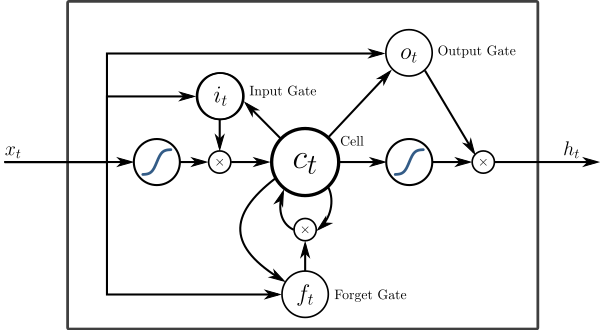
\includegraphics[width=50mm]{LSTM_wikipedia.png}
\caption{LSTM Model}
\label{fig:lstm}
\end{figure}

Figure~\ref{fig:lstm} shows the feed-back style of an LSTM. This image represents only one model of an LSTM (a peephole LSTM), but from the image, you can see that the current cell's output (ct) feeds back into the input to the (ct) layer. This means that the model trains on the current layer, but also retains information from previous layers. Since words in a sentence are related to the previous words, the LSTM is a model that fits well with text and document style data. For more information and for the source code to Keras' implementation the Keras LSTM model reference page can be found \href{https://keras.io/api/layers/recurrent_layers/lstm/}{here}. 




Note that here we are monitoring the categorical cross entropy loss and monitoring the total error and the accuracy. This allows us to see how accurate the model is becoming during training, and gives a metric that is more human understandable than loss values.


\subsection{Writing Inline One-Hot Encoding}

To do this, we need to replace the data keras generator to supply a new batch every time with the one-hot batch. This way we don't overwhelm the Colab notebook. Based on \href{https://github.com/keras-team/keras/issues/9707}{this Keras help page} we can get the format and necessary elements of the Generator.

\begin{verbatim}
## Keras has a native shuffler, but since our output isn't 
##one hot, we needto shuffle the data to ensure it 
## is the indexed item but one-hot-ified 
class Generator(Sequence):
    # Class is a dataset wrapper for better training performance
    def __init__(self, x_set, y_set, vocab_size, batch_size=128):
        self.x, self.y = x_set, y_set
        self.batch_size = batch_size
        self.indices = np.arange(self.x.shape[0]) 
        # all possible sequences
        self.vocab_size = vocab_size

    def __len__(self):
        return math.ceil(self.x.shape[0] / self.batch_size)

    def __getitem__(self, idx):
        value = self.batch_size:(idx + 1) * self.batch_size
        inds = self.indices[idx * value]
        indexed_x = self.x[inds] # sequences
        indexed_y = self.y[inds] # next_words

        # we need to do batching, so use bool 
        # to save space (we don't need an int)
        # it's one hot encoding so bool works fine
        # x =  [batch, seq_length, vocab_size]
        # y = [batch, vocab_size] 
        # for y it's just an array of sparse matricies,
        #so just convert it
        batch_y = np.asarray(indexed_y[0].todense())

        # for x, it's a little harder, since 
        # it's an array of 3 dense matricies
        # first convert it to a list, then convert 
        #it to a dense matrix, then 
        # convert it back into numpy array
        batch_x = []
        for batchidx, bat in enumerate(indexed_x): 
        # for every seq in the batch
            batch_x.append(bat[0].todense())
        batch_x = np.array(batch_x) 

        return batch_x, batch_y
    
    def on_epoch_end(self):
        np.random.shuffle(self.indices)

x = np.array(ohot_x)
y = np.array(ohot_y)
train_generator = Generator(x, y, VOCAB_SIZE)
\end{verbatim}

Essentially the only change we made to the original, is that we are forcing our x and y arrays into dense matricies. In the \_\_getitem\_\_ function. Keras naturally shuffles the dataset each epoch, so we are indexing into that item, and converting the one hot vectors for input and output to be a dense version. For the input vector, that is a [batch, seq\_length, vocab\_size] sized array, and for the label vector that is [batch, vocab\_size] in size.

Now that our data is ready to put into the model, let's call it by calling the generator class and putting that as the input to the model. 

\begin{verbatim}
model.fit(train_generator, epochs=EPOCHS, \
verbose=1, batch_size=BATCH_SIZE)
\end{verbatim}

\begin{figure}[h!]
\centering
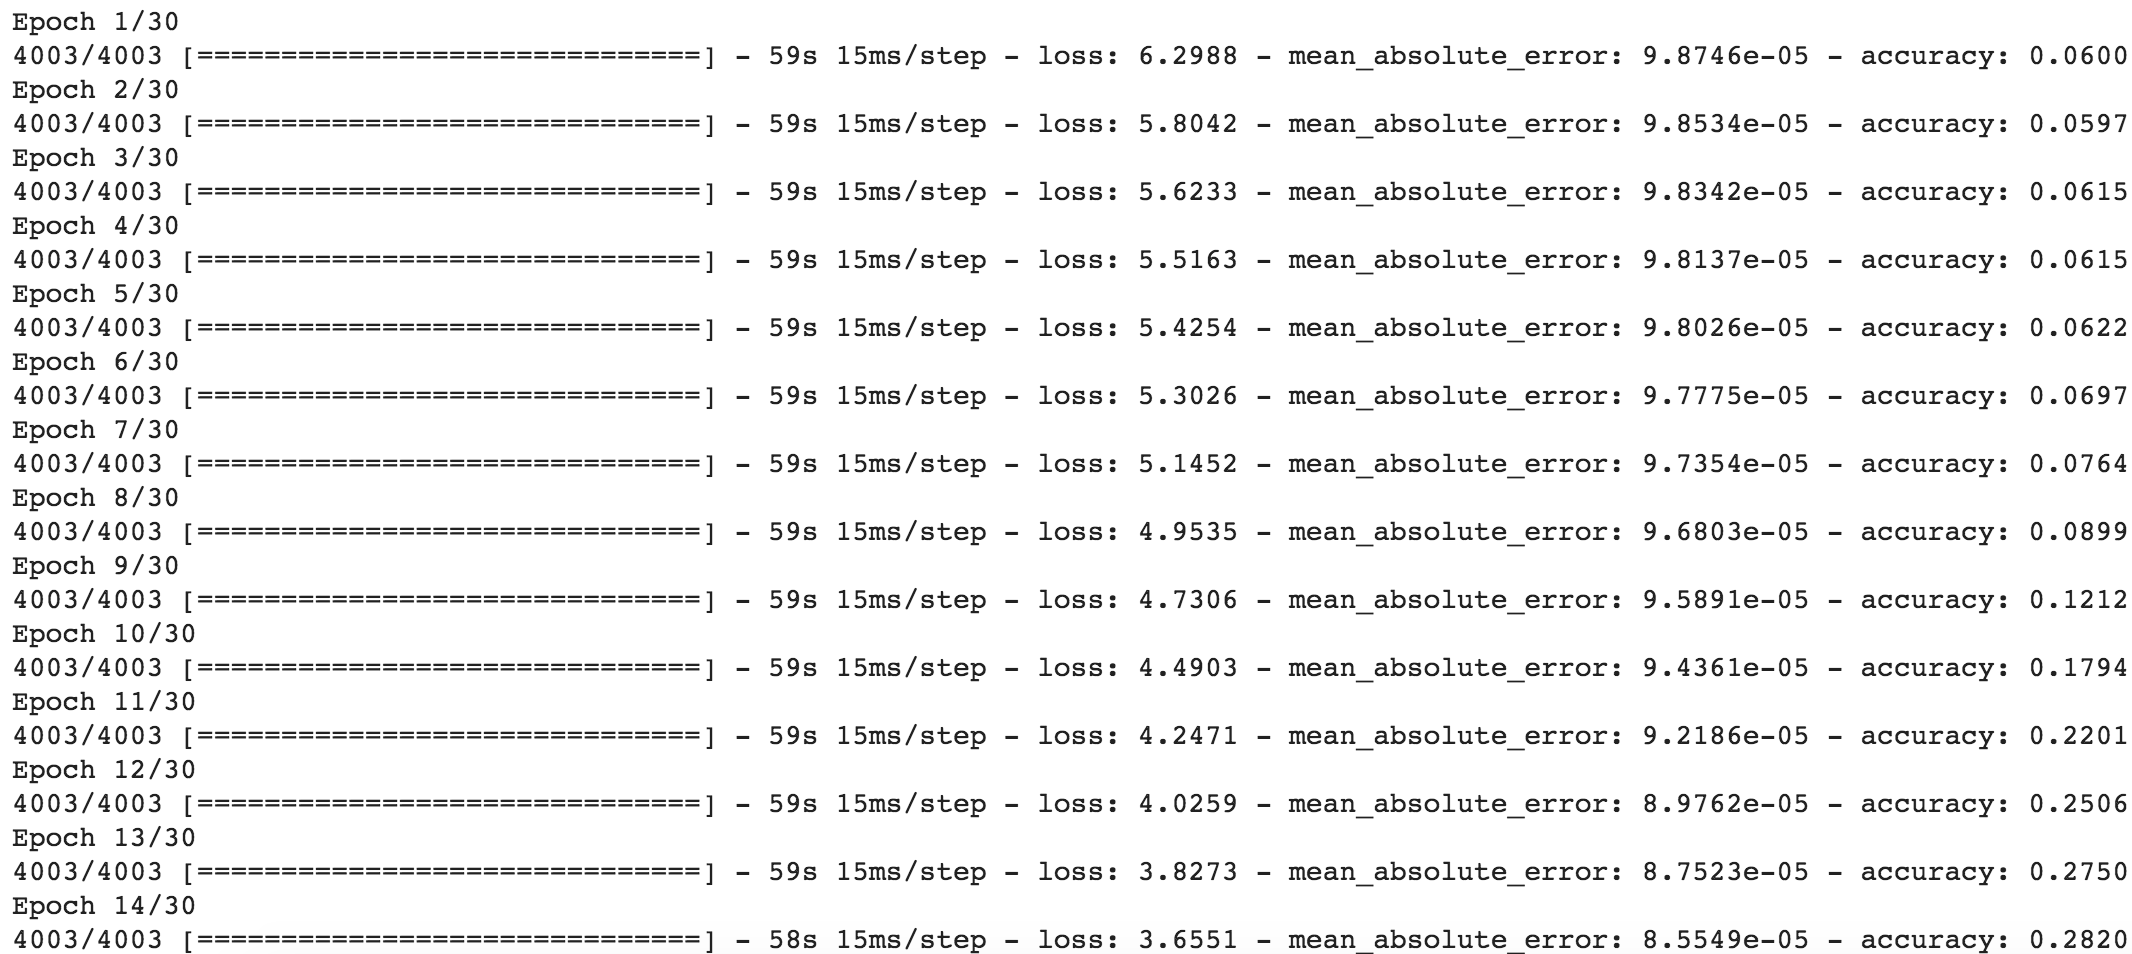
\includegraphics[width=50mm]{TrainingOutput.png}
\caption{Training Output From Model}
\label{fig:train}
\end{figure}

When we do that, you'll see outputs on the bottom of that Colab text box, they should look like Figure~\ref{fig:train}. This will allow you to monitor the progress of your training to verify that it is increasing in accuracy and decreasing in loss. 

If that's going really slow for you (likely). We can add a GPU to speed up the model.fit process.

 \subsection{Speed Up Using Tensor GPU}
 
 To use the GPU to train (this will save you so much time), attach a GPU to your Colab. To do this go to the Edit bar, and select Notebook Settings. From here you'll select GPU to run your network. TPUs require a lot of extra code to run, so make sure you select GPU, not TPU.
 
\begin{figure}[h!]
\centering
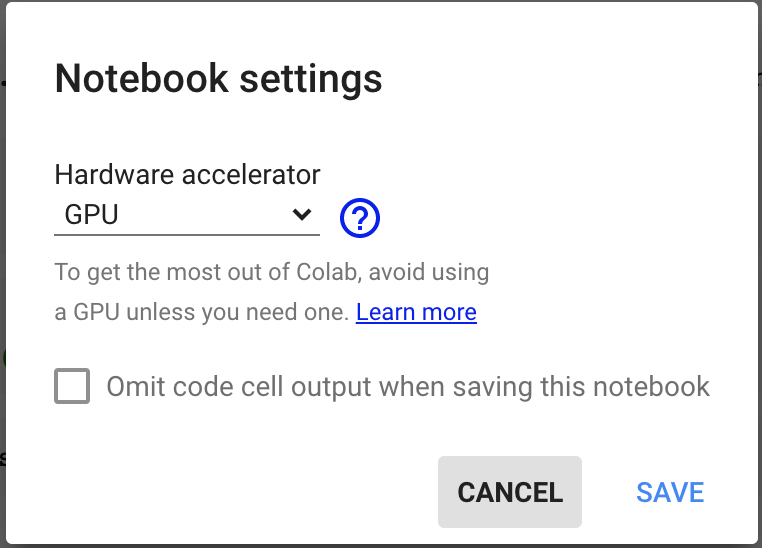
\includegraphics[width=50mm]{GPUAccel.png}
\caption{Use GPU to Accelerate Training}
\label{fig:gpu}
\end{figure}
 
 Since GPU is already enabled in Tensorflow 2.0 (the default Tensorflow Google Colab sources) you can run this like you would with a CPU. It does not require any changes to the code. 
  
  
  \subsection{Using Model Generate Text}
 We have a trained model, now we can generate text from it. To do this we want more than just one output word, so we are going to generate words in a function, and we are going to generate GENERATE\_LENGTH number of words. We're going to pick a randomly generated integer to get a word to start, then we are going to use the same random number to create a one-hot array, so the input matches the expected. Since we are only doing this on one index at a time, the space isn't an issue, so we can immediately force them to dense matrices. Doing that matches the expected input. From there, we will append the words into a list, and then join them together to make a sentence.  We are using .join(' ') to force it to add a space between each word returned from the list so it makes a sentence.
 
 
 \begin{verbatim}
# method for generating text
GENERATE_LENGTH = 20
def generate_text(model, length, text_size):
    # first get a random word as our starting point (input)
    ix     = [np.random.randint(text_size-SEQ_LENGTH) + SEQ_LENGTH]
    val    = [np.argmax(ohot_encoded[idx, :])]
    en     = encoder.inverse_transform(val)
    y_char = np.ndarray.tolist(en)

    # this is the output text, it'll be length long
    for i in range(length):
        #try:
        # one hot encode the current word
        X_words = []
        for n in range(SEQ_LENGTH):
          indexer = ix[0] - SEQ_LENGTH + n
          X = ohot_encoded[indexer, :]
          X = X.todense()
          X_words.append(X)
        X_words = np.array(X_words)
        #then the index changes to the predicted word 
        ix = [np.argmax(model.predict(X_words, 1))]
        val = [np.argmax(ohot_encoded[ix, :])]
        en  = encoder.inverse_transform(val)
        y_char.append(np.ndarray.tolist(en)[0])
        #except:
        #    continue

    # then combine all the words into a sentence        
    return (' ').join(y_char)

generate_text(model, GENERATE_LENGTH, len(allwords))
 \end{verbatim}
 
 This should write out generated text. Here is the example output text that mine gave:
 
 \begin{verbatim}
     must he mixed gregson pass to here said and her i of in 
     and still redskins horsemen falling to for refer
 \end{verbatim}
 
 Congratulations! You have now generated a document!
 
\end{document}

